\documentclass[a4 paper]{article}
\usepackage[inner=2.0cm,outer=2.0cm,top=2.5cm,bottom=2.5cm]{geometry}
\usepackage{setspace}
\usepackage[ruled]{algorithm2e}
\usepackage[rgb]{xcolor}
\usepackage{verbatim}
\usepackage{subcaption}
\usepackage{amsgen,amsmath,amstext,amsbsy,amsopn,tikz,amssymb,tkz-linknodes}
\usepackage{fancyhdr}
\usepackage[colorlinks=true, urlcolor=blue,  linkcolor=blue, citecolor=blue]{hyperref}
\usepackage[colorinlistoftodos]{todonotes}
\usepackage{rotating}
\usepackage{booktabs}
\newcommand{\ra}[1]{\renewcommand{\arraystretch}{#1}}

\newtheorem{thm}{Theorem}[section]
\newtheorem{prop}[thm]{Proposition}
\newtheorem{lem}[thm]{Lemma}
\newtheorem{cor}[thm]{Corollary}
\newtheorem{defn}[thm]{Definition}
\newtheorem{rem}[thm]{Remark}
\numberwithin{equation}{section}

\newcommand{\homework}[6]{
   \pagestyle{myheadings}
   \thispagestyle{plain}
   \newpage
   \setcounter{page}{1}
   \noindent
   \begin{center}
   \framebox{
      \vbox{\vspace{2mm}
    \hbox to 6.28in { {\bf MATH 118:~Statistics and Probability \hfill {\small (#2)}} }
       \vspace{6mm}
       \hbox to 6.28in { {\Large \hfill #1  \hfill} }
       \vspace{6mm}
       \hbox to 6.28in { {\it Instructor: {\rm #3} \hfill Name: {\color{teal}{Furkan \"OZEV\rm #5}} \hfill Student Id: {\color{teal}{161044036 \rm #6}}} \hfill}
       \hbox to 6.28in { {\it Assistant: #4  \hfill #6}}
      \vspace{2mm}}
   }
   \end{center}
   \markboth{#5 -- #1}{#5 -- #1}
   \vspace*{4mm}
}

\newcommand{\problem}[2]{~\\\fbox{\textbf{Problem #1}}\hfill (#2 points)\newline\newline}
\newcommand{\subproblem}[1]{~\newline\textbf{(#1)}}
\newcommand{\D}{\mathcal{D}}
\newcommand{\Hy}{\mathcal{H}}
\newcommand{\VS}{\textrm{VS}}
\newcommand{\solution}{~\newline\textbf{\textit{(Solution)}} }

\newcommand{\bbF}{\mathbb{F}}
\newcommand{\bbX}{\mathbb{X}}
\newcommand{\bI}{\mathbf{I}}
\newcommand{\bX}{\mathbf{X}}
\newcommand{\bY}{\mathbf{Y}}
\newcommand{\bepsilon}{\boldsymbol{\epsilon}}
\newcommand{\balpha}{\boldsymbol{\alpha}}
\newcommand{\bbeta}{\boldsymbol{\beta}}
\newcommand{\0}{\mathbf{0}}

\usepackage{graphicx}
\usepackage[utf8]{inputenc}
\usepackage{listings}
\lstset{
    language=Python,
    basicstyle=\ttfamily\small,
    aboveskip={1.0\baselineskip},
    belowskip={1.0\baselineskip},
    columns=fixed,
    extendedchars=true,
    breaklines=true,
    tabsize=4,
    prebreak=\raisebox{0ex}[0ex][0ex]{\ensuremath{\hookleftarrow}},
    frame=lines,
    showtabs=false,
    showspaces=false,
    showstringspaces=false,
    keywordstyle=\color[rgb]{0.627,0.126,0.941},
    commentstyle=\color[rgb]{0.133,0.545,0.133},
    stringstyle=\color[rgb]{01,0,0},
    numbers=left,
    numberstyle=\small,
    stepnumber=1,
    numbersep=10pt,
    captionpos=t,
    escapeinside={\%*}{*)}
}

\begin{document}
\homework{Homework \#4}{Due: 22/06/20}{Dr. Zafeirakis Zafeirakopoulos}{Gizem S\"ung\"u}{}{}
\textbf{Course Policy}: Read all the instructions below carefully before you start working on the assignment, and before you make a submission.
\begin{itemize}
\item It is not a group homework. Do not share your answers to anyone in any circumstance. Any cheating means at least -100 for both sides. 
\item Do not take any information from Internet.
\item No late homework will be accepted. 
\item For any questions about the homework, send an email to gizemsungu@gtu.edu.tr.
\item Submit your homework (both your latex and pdf files in a zip file) into the course page of Moodle.
\item Save your latex, pdf and zip files as "Name\_Surname\_StudentId".\{tex, pdf, zip\}.
\item The answer which has only calculations without any formula and any explanation will get zero. 
\item The deadline of the homework is 22/06/20 23:55.
\item I strongly suggest you to write your homework on \LaTeX. However, hand-written paper is still accepted \textbf{IFF} your hand writing is \textbf{clear and understandable to read}, and the paper is well-organized. Otherwise, I cannot grade your homework.
\item You do not need to write your Student Id on the page above. I am checking your ID from the file name.
\end{itemize}

\problem{1:}{10+10+10+10+10+10+40 = 100}
\textbf{WARNING:} Please show your OWN work. Any cheating can be easily detected and will not be graded.
\newline
\newline
For the question, please follow the file called airplane\_crashes.txt while reading the text below.\\
\newline
In each year from 1993 to 2012, the number of airplane crashes in airline companies were counted. The data was collected from 14 different airline companies. The numbers of crashes for the airline companies are indicated in 14 columns following the year column. Assume that the number of crashes per airline company per year is a random variable having a Poisson($\lambda$) and that the number of crashes in different airline company or in different years are independent.\\
(Note: You should implement a code for your calculations for each following subproblem. You are free to use any programming languages (Python, R, C, C++, Java) and their related library.)

\subproblem{a} Give a table how many cases occur for all companies between 1993 and 2012 for each number of crashes (\# of Crashes).\\
Hint: When you check the file you will see: \# of Crashes = \{0, 1, 2, 3, 4\}.\\
\begin{table}[htb!]
	\centering
	\begin{tabular}{c|c}
		\begin{tabular}[c]{@{}c@{}}\textbackslash{}\# of\\Crashes\end{tabular} & \begin{tabular}[c]{@{}c@{}}\textbackslash{}\# of cases\\in all company \\between the years\end{tabular}  \\ 
		\hline
		0                                                                      &       144                                                                                                   \\
		1                                                                      &        91                                                                                                  \\
		2                                                                      &        32                                                                                                  \\
		3                                                          & 11
		\\
		4                                                                      &        2                                                                                                
	\end{tabular}

\caption{Actual cases}
\label{tab1}
\end{table}
\newpage

\subproblem{b} Estimate $\lambda$ from the given data. \\
{\color{olive} $\blacklozenge$ The Poisson parameter Lambda is the total number of events (k) divided by the number of units (n) in the data ( lambda = k/n)} \\
{\color{olive} $\blacklozenge$ So, Lambda ($\lambda$) = total number of crashes / total number of cases} \\
{\color{violet} $\blacklozenge$ total number of crashes = (0 * 144) + (1 * 91) + (2 * 32) + (3 * 11) + (4 * 2) = 196}\\
{\color{violet} $\blacklozenge$ total number of cases = 144 + 91 + 32 + 11 + 2 = 280}\\
{\color{teal} So, Lambda ($\lambda$) = 196 $/$ 280 = 0.7 } \\
\subproblem{c} Update Table \ref{tab1} in Table \ref{tab2} with Poisson predicted cases with the estimated $\lambda$.\\
\begin{table}[htb!]
	\centering
	\begin{tabular}{c|c|c}
		\begin{tabular}[c]{@{}c@{}}\textbackslash{}\# of\\Crashes\end{tabular} & \begin{tabular}[c]{@{}c@{}}\textbackslash{}\# of cases\\in all companies\\between the years\end{tabular} & \begin{tabular}[c]{@{}c@{}}Predicted \textbackslash{}\# of cases\\in all companies\\between the years\end{tabular}  \\ 
		\hline
		0                                                                      &        144                                                                                                  &          139                                                                                                           \\
		1                                                                      &    91                                                                                                      &           97                                                                                                          \\
		2                                                                      &     32                                                                                                     &            34                                                                                                         \\
		3                                                                      &      11                                                                                                    &    8
		\\
		4                                                                      &     2                                                                                                     &           1                                                                                                       
	\end{tabular}
\caption{Actual vs. Predicted Cases}
\label{tab2}
\end{table}
\newline \subproblem{d} Draw a barplot for the actual cases (Table \ref{tab2} in column 2) and the predicted cases (Table \ref{tab2} column 3) with respect to \# of crashes. You should put the figure.\\
\newline 
\begin{figure}
  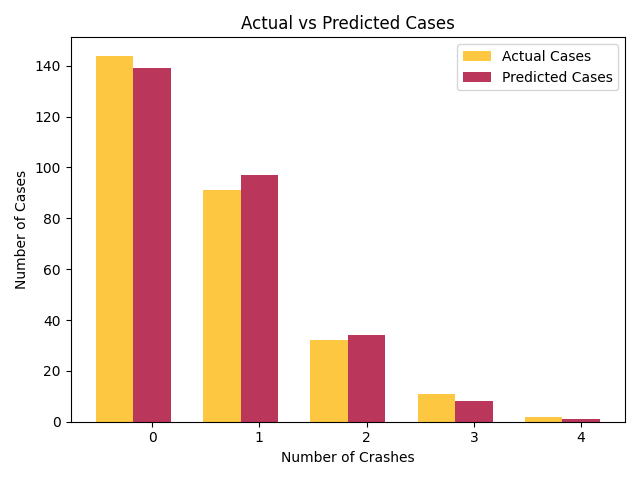
\includegraphics[scale=1]{Figure.png}
  \caption{A barplot.}
  \label{fig:barplot}
\end{figure}
\newpage
\subproblem{e} According to the barplot in (c), does the poisson distribution fit the data well? Compare the values of the actual cases and the values of the poisson predicted cases, and write your opinions about performance of the distribution.\\
\newline {\color{olive} $\blacklozenge$ To determine if the poisson distribution fits the data well, it is necessary to compare the actual cases with the predicted cases.} \\
\newline {\color{teal} Total number of actual cases: 144 + 91 + 32 + 11 + 2 = 280}
\newline {\color{teal} Total number of predicted cases: 139 + 97 + 34 + 8 + 1 = 279} \\
\newline {\color{violet} As we have seen, the distribution data do not fit exactly, but we can say that it fits well enough.}
\newline {\color{violet} Because there is no serious difference.}
\newline {\color{violet} This difference is due to rounding to the nearest decimal.} \\
\newline {\color{olive} Actual case and predicted case numbers are very close to each other.}
\newline {\color{olive} When we evaluate in terms of performance, it can make very close prediction using Poisson distribution.}
\newline {\color{olive} Using the Poisson distribution can be efficient in terms of creating a predicted distribution data.} \\
\subproblem{f} According to your estimations above, write your opinions considering your barplot and Table \ref{tab2}. Do you think that airplane transportation is dangerous for us? Whether yes or no, explain your reason.\\
\newline {\color{olive} $\blacklozenge$ In order to decide that air transport is dangerous for us, we need to compare and interpret the numbers of real cases and predicted cases.} \\
\newline {\color{teal} Based on the actual number of cases, 144 cases never had an crashes.}
\newline {\color{teal} Based on the predicted number of cases, there will never be a crash in 139 cases.} \\
\newline {\color{teal} Based on the actual number of cases, 196 crashes occurred. ((91 * 1) + (32 * 2) + (11 * 3) + (4 * 2) = 196)}
\newline {\color{teal} Based on the predicted number of cases, 191 accidents will occur. ((97 * 1) + (34 * 2) + (8 * 3) + (1 * 2) = 191)} \\
\newline {\color{teal} Based  on  the  actual  number  of  cases, the crash-free rate is 0.424 (144 / (144 + 196) = 0.424).}
\newline {\color{teal} Based  on  the  predicted  number  of  cases, the crash-free rate is 0.421 (139 / (139 + 191) = 0.421).} \\
\newline {\color{violet} As can be seen, the rate of no crash-free has decreased according to the predicted data. (0.424 $>$ 0.421)}
\newline {\color{violet} Therefore, we can say that the risk of crashes increased.}
\newline {\color{violet} When we interpret according to the predicted data, we can say that airplane transportation is not safe.}
\newline {\color{violet} So, answer is yes.} 
\newpage
\subproblem{g} Paste your code that you implemented for the subproblems above. Do not forget to write comments on your code.\\
Example:\\
\begin{itemize}
	\item The common code block for all subproblems\\
	
	\begin{lstlisting}[label={list:first},caption=The common code - Import modules and File operations]
from tabulate import tabulate
import math
import numpy as np
import matplotlib.pyplot as plt

if __name__ == '__main__':

	# Open file
	file = open("airplane_crashes.txt")

	# Read all context from file
	line = file.read()
	
	# Close file
	file.close()
    \end{lstlisting}
	
	\item The code block for (a)\\
	
		\begin{lstlisting}[label={list:first},caption=The code block a - Compute the values in Table 1 and Print table]
	
	# Create a dictionary structure to keep crashes
	cases = dict()

	# Split lines
	line = line.split('\n')

	for cline in line:

		# Split line with tab, because there is tab among the numbers.
		item = cline.split('\t')

		# For each column except first and second column
		for i in item[2:]:
			# convert string to integer number
			x = int(i)
			# If number exists in dictionary, increment by 1.
			if x in cases:
				cases[x] += 1
			# Else, add new key with value 1.
			else:
				cases[x] = 1

	# For print table 1
	table1=[["\\# of Crashes","\\# of cases in all company between the years"]]

	for i in cases:
		table1.append([i, cases[i]])

	print("\n(a)\t\t\tTABLE 1: Actual cases")
	print(tabulate(table1, headers="firstrow", tablefmt='orgtbl'))
\end{lstlisting}
	
	\item The code block for (b)\\
	
		\begin{lstlisting}[label={list:first},caption=The code block b - Compute Lambda]
	
	sum = 0
	count = 0

	for i in cases:
		# Calculate total number of cases
		count += cases[i]
		# Calculate total number of crashes
		sum += cases[i] * i

	# The Poisson parameter Lambda is the total number of events (k) divided by
	# the number of units (n) in the data ( lambda = k/n)
	# So, Lambda = total number of crashes / total number of cases
	lambdaa = sum / count

	print("\n(b) Lambda: {}\n". format(lambdaa))
\end{lstlisting}
	
	\item The code block for (c)\\
	
		\begin{lstlisting}[label={list:first},caption=The code block c - Compute the values in Table 2 and Print table]

	predict_case = dict()
	table2 = [["\\# of Crashes","\\# of cases in all company between the years"
			,"Predicted \\# of cases in all companies between the years"]]

	for i in cases:
		# Poisson formula applied.
		# Then, the result was multiplied by the total number of cases.
		# round () function was used to round the result to the nearest decimal.
		predict_case[i] = pow(math.e, -1*lambdaa) * pow(lambdaa, i)
		predict_case[i] /= math.factorial(i)
		predict_case[i] *= count
		predict_case[i] = round(predict_case[i])

		table2.append([i, cases[i], predict_case[i]])

	# For print table 2
	print("(c)\t\t\t\t\tTABLE 2: Actual vs. Predicted Cases")
	print(tabulate(table2, headers="firstrow", tablefmt='orgtbl'))
\end{lstlisting}
	
	\item The code block for (d)\\
	
		\begin{lstlisting}[label={list:first},caption=The code block d - Draw the barplot]

	caselist = list()
	predictlist = list()

	# Create actual and predict list.
	for i in cases:
		# Take value from dictionary structure, and add these lists.
		caselist.append(cases[i])
		predictlist.append(predict_case[i])

	# Number of crashes, like 0,1,2,3,4
	n_groups = len(cases)
	nlist = list()
	for i in range(n_groups):
		nlist.append(i)

	# Create barplot for the actual cases
	# and the predicted cases with respect to # of crashes.
	fig, ax = plt.subplots()
	index = np.arange(n_groups)
	bar_width = 0.35
	opacity = 0.8

	# Give actual and predicted case lists.
	rects1 = plt.bar(index, caselist, bar_width, alpha=opacity,
			 color='#fdb912', label='Actual Cases')

	rects2 = plt.bar(index + bar_width, predictlist, bar_width, alpha=opacity,
			color='#a90432', label='Predicted Cases')

	# Determine labels.
	plt.xlabel('Number of Crashes')
	plt.ylabel('Number of Cases')
	plt.title('Actual vs Predicted Cases')
	plt.xticks(index + bar_width, nlist)
	plt.legend()

	plt.tight_layout()
	# Show barplot
	plt.show()
\end{lstlisting}
	
\end{itemize}




\end{document} 


